%\documentclass[12pt,a4paper,addpoints]{exam}
\documentclass[12pt,a4paper,addpoints,answers]{exam}
\usepackage[T1]{fontenc}
\usepackage[utf8]{inputenc}
\usepackage[spanish]{babel}
\usepackage{adjustbox}
\usepackage{multirow}
\usepackage{graphicx}
\usepackage{minted}
\usepackage{tikz}
\usepackage{amsmath}
\usepackage{setspace}
\usepackage{afterpage}
\usepackage{wrapfig}


% Términos en castellano
\pointpoints{Punto}{Puntos}
\bonuspointpoints{Punto extra}{Puntos extra}
\renewcommand{\solutiontitle}{\noindent\textbf{Solución propuesta:}\enspace\\}
\chqword{Pregunta}
\chpgword{Página}
\chpword{Punto}
\chbpword{Punto extra}
\chsword{Obtenidos}
\chtword{Totales}
\hpword{Puntos:}
\hsword{Nota:}
\hqword{Bloque:}
\htword{Total:}

\pagestyle{headandfoot}
\firstpageheadrule
\runningheadrule
\firstpageheader{Bases de Datos I}{}{Convocatoria ordinaria\\Curso 2023/2024}
\runningheader{Bases de Datos I}{}{Convocatoria ordinaria\\Curso 2023/2024}
\firstpagefooter{}{}{\thepage\,/\,\numpages}
\runningfooter{}{}{\thepage\,/\,\numpages}

\begin{document}

\begin{table}[t]
\renewcommand{\arraystretch}{1.2}
\small
\centering
\begin{tabular}{|l|p{5.5cm}|p{5.cm}|}
\hline
\multirow{3}{*}{
\includegraphics[width=2.5cm]{logos/etsisi}} & \multicolumn{2}{l|}{Apellidos:} \\ \cline{2-3} 
                  & \multicolumn{2}{l|}{Nombre:}    \\ \cline{2-3} 
                  & DNI:  & Num. mat.: \\ \hline
\end{tabular}%
\label{tab:datos}
\end{table}

%\begin{center}
%\gradetable[h][questions]
%\end{center}

\begin{center}\textbf{Normativa de examen}\end{center}
\begin{itemize}
    \item No está permitido el uso de dispositivos móviles ni otros dispositivos electrónicos.
    \item Cada estudiante podrá disponer de un folio tamaño A4 con las anotaciones que considere oportunas para desarrollar su examen. El folio podrá contener texto por ambas caras.
    \item Durante el examen, el profesor podrán solicitar acreditar la identidad de los participantes en el mismo. Deberá tener en todo momento su Documento Nacional de Identidad y/o Carné de la UPM visible sobre la mesa.
    \item El examen deberá estar escrito en bolígrafo de color azul o negro.
    \item No se permite abandonar el aula de examen durante los primeros 15 minutos. Transcurrido este tiempo, no se permitirá entrar al examen. 
    \item El examen tiene una duración máxima de \textbf{2.5 horas}. 
    \item Justifique sus respuestas lo mejor posible indicando, si fuese necesario, los pasos realizados.
    \item Las calificaciones provisionales serán publicadas en el Moodle de la asignatura el viernes 14 de junio de 2024.
    \item La fecha para la revisión del examen se anunciará en el Moodle de la asignatura junto a la publicación de las calificaciones.
\end{itemize}

\vspace{1cm}

\begin{center}
\gradetable[h][questions]
\end{center}

\newpage


\begin{questions}

% Bloque 1: Modelo Entidad/Relación y paso a tablas
\question{\textbf{Bloque ``Modelo Entidad/Relación y paso a tablas''}}

\begin{parts}
\part[3]

En un lugar algo olvidado de la red, donde paquetes TCP y UDP hacen cola y los hackers de sombrero negro acechan en las sombras, se encuentra la gran corporación \textit{ByteMagic Inc}.

Tras un viernes de actualizaciones en sus sistemas (tarea que según algunos empleados tuvo más de \textit{magic} que de \textit{bytes}), los ingenieros comenzaron a idear lo que terminaron denominando \textbf{La Fortaleza}. Esta maravilla de la seguridad se concibió para mantener a raya a los intrusos y proteger los valiosos datos de la compañía incluyendo, por supuesto, la colección de memes de los de DevOps.

\textbf{La Fortaleza} estaría organizada en niveles, como las capas de una cebolla muy temperamental. Cada nivel contendría uno o más centros de control con nombre en clave único, fortificados con un tipo de \textit{firewall}, por lo que sería necesario saber tanto qué software tiene instalado como su versión.

Los guardas estarían meticulosamente identificados y jerarquizados. Cada uno de ellos, salvo el Comandante en Jefe, podrá tener una banda de subordinados a su cargo, cual gallinas bajo el ala protectora de otra gallina, aunque esta más grande y ligeramente paranoica. Los guardas tendrían la noble misión de proteger, al menos, un nivel. Además, cada centro de control contaría con un único guarda responsable para asegurar de que todo funciona como un reloj suizo.

En caso de que el caos decidiera hacer una visita, los guardas pueden dirigirse a los depósitos de armas (también cada uno con su nombre en clave) que hay repartidos por los niveles, ya que todos los niveles tienen al menos uno de estos arsenales al lado de la cafetería. Allí, se pertrecharían con todos los tipos de arma que quisieran, pero no sin antes cumplir con el tedioso pero necesario protocolo: el registro meticuloso sobre qué tipo de arma han tomado, la fecha y hora exactas de retirada y, por supuesto, la fecha y hora de la devolución en el momento que la devuelvan. Porque en la fortaleza, hasta el caos se maneja con un orden impecable y un desmedido amor por el papeleo.

\textbf{realizar} un modelo conceptual de datos mediante la técnica del \textbf{modelo Entidad-Relación de Chen} que modele \textbf{La Fortaleza}.


\begin{solution}
    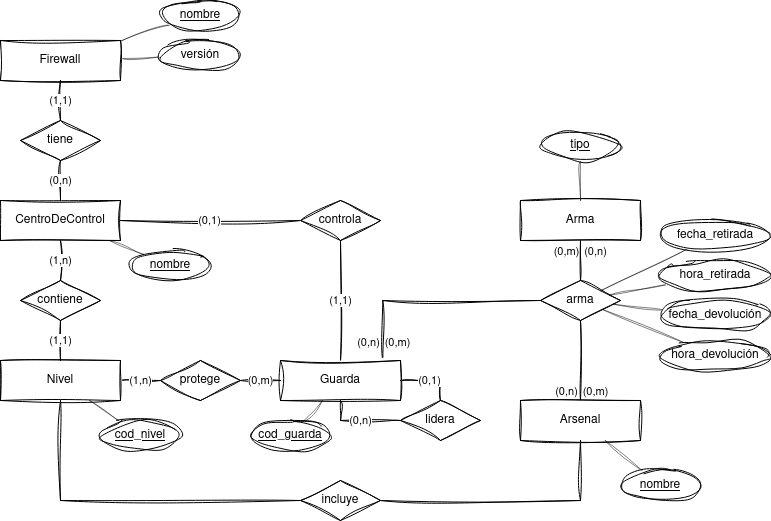
\includegraphics[width=\textwidth]{figs/2024-ordinaria-gcdia-mer.png}
\end{solution}
\end{parts}


% SQL
\newpage
\question{\textbf{Bloque ``SQL''}}

Dado el siguiente modelo relacional:

\texttt{CRIATURA (\underline{Nombre}, Sexo, Especie)}

\texttt{TRATAMIENTO (\underline{Nombre}, Descripción, Enfermedad)}

\texttt{PERSONAL (\underline{Nombre}, Sexo, Especialidad, Rol)}

\texttt{APLICA (\underline{\emph{Criatura}}, \underline{\emph{Tratamiento}}, \underline{\emph{Personal}}, Fecha, Hora)}

Se pide:
\begin{parts}

% resta
\part[\half] Escriba una consulta en SQL que devuelva el \texttt{nombre} de las criaturas que nunca han recibido un \texttt{tratamiento} cuyo \texttt{nombre} sea `\textit{tónico de bailes}'.

\begin{solution}[15em]
\begin{minted}[baselinestretch=1,fontsize=\small]{sql}
SELECT nombre
FROM critura
WHERE nombre NOT IN (SELECT critaura
                     FROM aplica
                     WHERE tratamiento = 'tónico de bailes')
\end{minted}
\end{solution}

% interseccion
\part[\half] Escriba una consulta en SQL que devuelva el \texttt{nombre} del personal que ha aplicado algún tratamiento a las criaturas cuyo \texttt{nombre} sea `\textit{Risueño Rob}' y `\textit{Caféinomano Eduardo}'.

\begin{solution}[15em]
\begin{minted}[baselinestretch=1,fontsize=\small]{sql}
SELECT nombre
FROM personal
WHERE nombre IN (SELECT personal
                 FROM aplica
                 WHERE criatura = 'Risueño Rob')
  AND nombre IN (SELECT personal
                 FROM aplica
                 WHERE criatura = 'Cafeinómano Eduardo')         
\end{minted}
\end{solution}

% division
\part[\half] Escriba una consulta en SQL que devuelva el \texttt{nombre} del tratamiento que se haya aplicado a todas las criaturas de la \texttt{especie} `\textit{zombi}'.

\begin{solution}[15em]
\begin{minted}[baselinestretch=1,fontsize=\small]{sql}
SELECT nombre
FROM tratamiento
WHERE NOT EXISTS (SELECT *
                  FROM criatura
                  WHERE especie = 'zombi'
                    AND NOT EXISTS (SELECT *
                                    FROM aplica
                                    WHERE aplica.tratamiento = 
                                            tratamiento.nombre
                                      AND aplica.criatura = 
                                            criatura.nombre))
\end{minted}
\end{solution}

% maximo
\part[\half] Escriba una consulta en SQL que devuelva el \texttt{nombre} del tratamiento o tratamientos más veces aplicado.

\begin{solution}[15em]
\begin{minted}[baselinestretch=1,fontsize=\small]{sql}
SELECT tratamiento
FROM aplica
GROUP BY tratamiento
HAVING COUNT(*) >= ALL (SELECT COUNT(*)
                        FROM aplica
                        GROUP BY tratamiento);
\end{minted}
\end{solution}

% joins
\part[\half] Escriba una consulta en SQL que devuelva el \texttt{nombre} de las criaturas de la \texttt{especie} `\textit{sirena}' a las que se le haya aplicado algun tratamiento por personal de la \texttt{especialidad} `\textit{Pociones de la Eternidad}'.

\begin{solution}[15em]
\begin{minted}[baselinestretch=1,fontsize=\small]{sql}
SELECT DISTINCT criatura.nombre
FROM aplica
    INNER JOIN criatura ON criatura.nombre = aplica.criatura
    INNER JOIN personal ON personal.nombre = aplica.personal
WHERE criatura.especie = 'sirena'
  AND personal.especialidad = 'Pociones de la Eternidad';
\end{minted}
\end{solution}

% procedmiento
\part[1] Escriba un procedimiento almacenado en SQL que dado el nombre de una \texttt{enfermedad}, que se pasará como parámetro de entrada, liste por pantalla el número de veces que se han aplicado tratamientos para dicha enfermedad a cada \texttt{especie}. Si una especie nunca ha recibido tratamientos no es necesario que aparezca en el listado. El listado debe aparecer ordenador de mayor a menor número de tratamientos aplicados.

\begin{solution}[15em]
\begin{minted}[baselinestretch=1,fontsize=\small]{sql}
DELIMITER $$
CREATE PROCEDURE num_tratamientos_especie (IN enf VARCHAR(30))
BEGIN
    SELECT criatura.especie, COUNT(*) AS num_veces
    FROM aplica
        INNER JOIN criatura ON criatura.nombre = aplica.criatura
        INNER JOIN tratamiento ON tratamiento.nombre = aplica.tratamiento
    WHERE tratamiento.enfermedad = enf
    GROUP BY criatura.especie
    ORDER BY num_veces DESC;
END$$
DELIMITER ;
\end{minted}
\end{solution}

% trigger
\part[1] Escriba un \textit{trigger} en SQL que impida que se inserten nuevas aplicaciones de tratamiento a criaturas si ya se han aplicado antes aunque sean realizadas por personal diferente.

\begin{solution}[15em]
\begin{minted}[baselinestretch=1,fontsize=\small]{sql}
DELIMITER $$
CREATE TRIGGER evita_tratamiento_duplicado BEFORE INSERT ON aplica 
FOR EACH ROW
BEGIN
    DECLARE num_trat INTEGER;

    SELECT COUNT(*) INTO num_trata
    FROM aplica
    WHERE criatura = NEW.criatura
      AND tratamiento = NEW.tratamiento;

    IF num_trata > = THEN
        SIGNAL SQLSTATE '481516'
        SET MESSAGE_TEXT = 'No se puede aplicar dos veces el mismo 
        tratamiento';
    END IF;
END$$
DELIMITER ;
\end{minted}
\end{solution}

% vista con usuario
\part[1] Cree una vista en SQL que permita conocer el número de tratamientos aplicado por cada personal (las columnas de la vista deberán ser el \texttt{nombre} del personal y el número total de tratamiento aplicados). A continuación, cree un usuario denominado `\textit{gerente}' que tenga únicamente permisos de consulta sobre esa vista.

\begin{solution}[12em]
\begin{minted}[baselinestretch=1,fontsize=\small]{sql}
CREATE VIEW num_tratamientos_personal AS
SELECT personal, COUNT(*) AS num_tratamiento
FROM aplica
GROUP BY personal;

CREATE USER 'gerente' IDENTIFIED BY '1234';

GRANT SELECT ON num_tratamientos_personal TO 'gerente';
\end{minted}
\end{solution}

\end{parts}


% Bloque Acceso programático
\newpage
\question{\textbf{Bloque ``Acceso programático''}}

\begin{parts}
\part[1] Tomando como punto de partida un \texttt{SCHEMA} de bases de datos basado en el modelo relacional del bloque anterior, complete los huecos del siguiente código fuente en \texttt{python} de tal manera que se satisfaga la funcionalidad indicada como comentarios.

\begin{minted}[baselinestretch=1,fontsize=\small]{python}
import mysql.connector

# establecimiento de conexion
mydb = mysql.connector.connect(
  host="localhost",
  user="root",
  password="root"
)

cursor = mydb.cursor()

# añade personal
nombre = "Atenea la Moderada"
sexo = "M"
especialidad = "Curación de Maldiciones Graves"
rol = "Asistente"

cursor.execute("INSERT INTO personal _________________________________",
    (nombre, sexo, especialidad, rol))

mydb.commit()

# listar los nombres y sexo de las criaturas de especie "fénix"
especie = "fénix"
consulta = "SELECT nombre, sexo FROM criatura WHERE especie = %s"

cursor.______________(________________________________________________)

for (nombre, sexo) in cursor:
    print(f"{nombre} ({sexo})")

# cierre de recursos
cursor.close()
cnx.close()
mydb.close()

\end{minted}

\begin{solution}[1em]
\begin{minted}[baselinestretch=1,fontsize=\small]{python}
import mysql.connector

# establecimiento de conexion
mydb = mysql.connector.connect(
  host="localhost",
  user="root",
  password="root"
)

cursor = mydb.cursor()

# añade personal
nombre = "Atenea la Moderada"
sexo = "M"
especialidad = "Curación de Maldiciones Graves"
rol = "Asistente"

cursor.execute("INSERT INTO personal VALUES (%s, %s, %s, %s)",
    (nombre, sexo, especialidad, rol))

mydb.commit()

# listar los nombres y sexo de las criaturas de especie "fénix"
especie = "fénix"
consulta = "SELECT nombre, sexo FROM criatura WHERE especie = %s"

cursor.execute(consulta, (especie,))

for (nombre, sexo) in cursor:
    print(f"{nombre} ({sexo})")

# cierre de recursos
cursor.close()
cnx.close()
mydb.close()
\end{minted}
\end{solution}

\end{parts}

% Bloque Acceso seguro
\newpage
\question{\textbf{Bloque ``Acceso seguro''}}

\begin{parts}

\part[\half] Explique brevemente en qué consiste un ataque de \textit{SQL Injection}

\begin{solution}[15em]
Un ataque de \textit{SQL Injection} es cuando un hacker inserta código malicioso en los campos de entrada de una aplicación web. Si la aplicación no filtra o valida correctamente estos datos, el código malicioso se ejecuta en la base de datos y el atacante puede obtener acceso no autorizado, robar información o manipular la base de datos. Para prevenir estos ataques, es importante que los desarrolladores implementen medidas de seguridad como el filtrado de entradas y el uso de consultas preparadas.
\end{solution}

\end{parts}

\end{questions}
\end{document}
